\section{Columnar Data Storing}

The final stage of any data analysis is representing the data in a columnar format and fetching some subset of the data with constraints 
on other columns. At this stage, users operate on a large data set with many columns and rows, and access to all of the 
columns in the file is not required. The Apache Parquet format is widely used in data science for storing columnar data, due to its tools
with Python data frames. It is highly tuned to store large data sets and provide fast access to required columns. The Parqute is gaining
some popularity in High Energy and Nuclear Physics with the growing popularity of Python as a physics analysis environment. In the
past two decades, the ROOT was the primary tool for physics analysis which also provides data structures for storing columnar data 
and accessing the columns selectively. It is worth mentioning that ROOT also has Python bindings. 

\subsection{Design}

The flexibility of the HiPO data format allows storing data in columnar format, similar to Parquete and ROOT. 
The feature of assigning tags to records allows for writing the data in a columnar manner, where each column is assigned a tag and written separately into its own record.
This process is synchronized so that at every predetermined number of rows, every column data is serialized and outputted as a record. The schematic view of arranging 
the data in the file is shown in Figure~\ref{fig:tuple_schema}.

\begin{figure}[h!]
  \begin{center}
    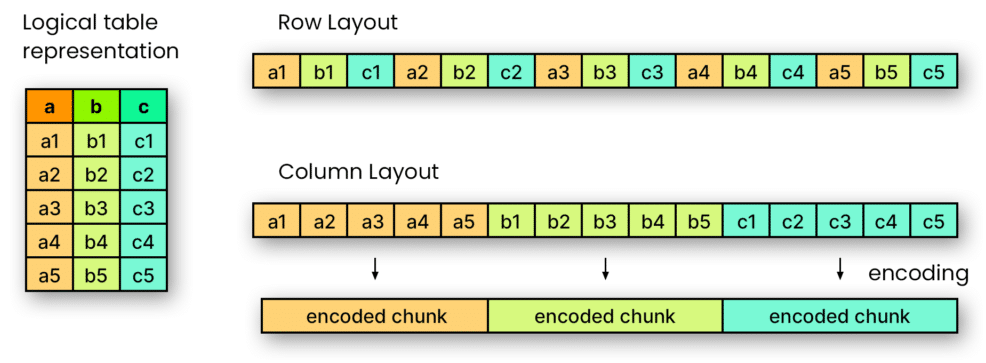
\includegraphics[width=0.85\textwidth]{images/tuple_schema.png}
 \end{center}
  \caption{Schematic view of arranging each event in the file from columnar table.}
 \label{fig:tuple_schema}
\end{figure}

When reading the file, the desired columns (called branches) are declared, and only records (buckets) with corresponding tag numbers are read and deserialized.
The user program has access only to the declared branches. The files written as columnar data have to be read with the corresponding API to make sure that the columns 
are properly synchronized at the read time. Here is an example code to read a few columns from a file and fill histogram. 
%\begin{verbatim}
\rule{16.5cm}{0.4pt}
\begin{lstlisting}[language=c++, caption=c++ example to read tuple file and fill histogram.]
// open file and read only specified branches
hipo::tuple tuple("tuple.h5", "c1:c2:c3:c4"); 
float data[4]; // declare a holder for the data to be read
twig::h1d h(120,-1.0,1.0); // declare a histogram
while(tuple.next(data)==true){
    h.fill(data[0]);
}
\end{lstlisting}
%\end{verbatim}

The example code code opens a file to read branches names "c1"-"c4" from the file, reads all rows until reaching the end of the file passing them to the user code through a declared array.
The values from the first branch (which is "c1") will be filled into a histogram.

\subsection{Benchmarking}

For reading tests, we produced a synthetic data set consisting of 24 columns and 50 M rows and created HiPO (4.8 GB), ROOT (4.4 GB), and Parquete (5.1 GB) all three with 
LZ4 compression. The columns were filled with random numbers generated by the Java Random class with a Gaussian distribution with a standard deviation of 1.0. 

\begin{figure}[h!]
  \begin{center}
    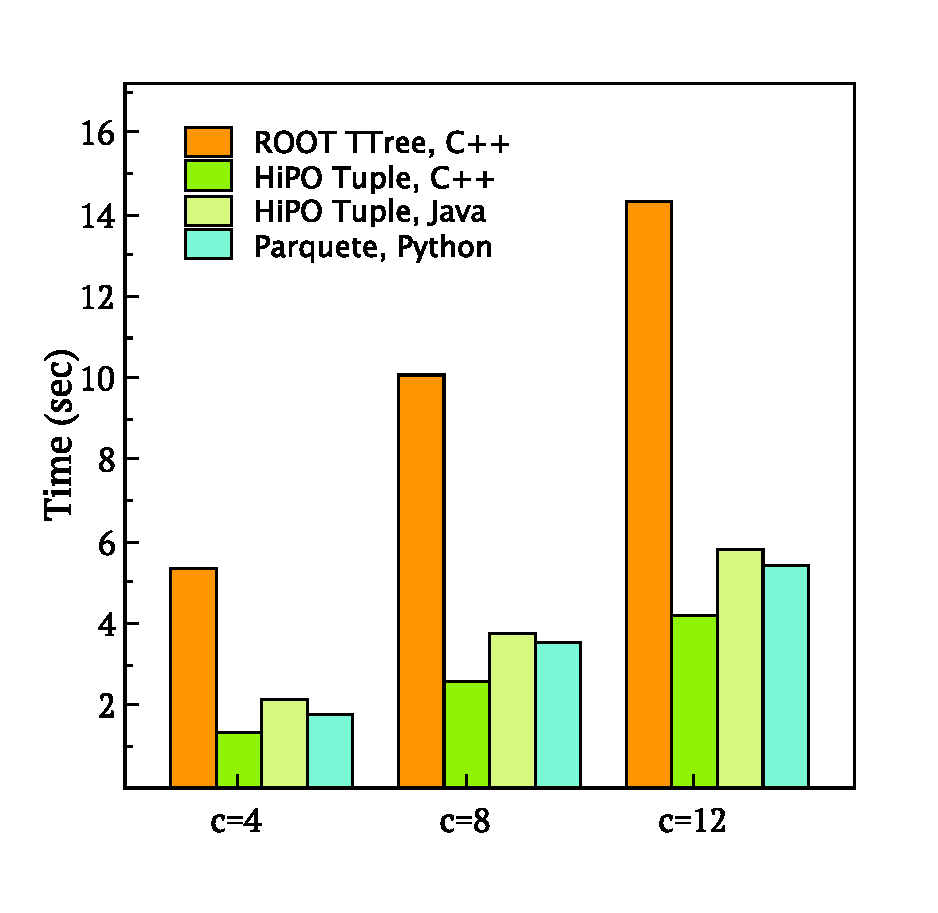
\includegraphics[width=0.45\textwidth]{images/read_benchmark.pdf}
     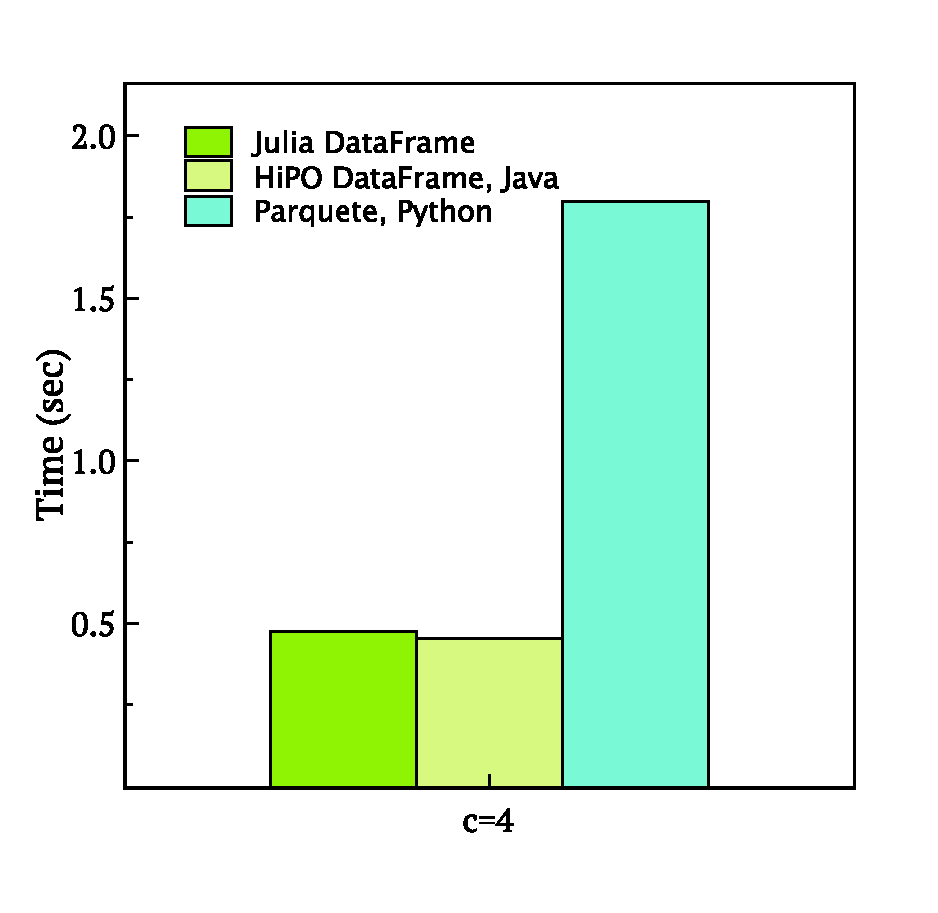
\includegraphics[width=0.45\textwidth]{images/data_frame_benchmark.pdf}
 \end{center}
  \caption{Reading benchmark for different file formats reading the same data with 24 columns and 50 M rows. Nd - is the number of columns that are read from the file, and a histogram is filled for each column. }
 \label{read_benchmark}
\end{figure}

Then, reading tests were performed by reading 4, 8, and 12 branches (out of 24) from the data file and filling a histogram for each branch, representing a typical workflow for data exploration. The times were measured for ten consecutive reads, and the average time of the last four reads was used as the final result. The results are shown in Figure~\ref{read_benchmark}. As can be seen from the figure the ROOT TTree has the worst performance. The C++ HiPO library has the best read times, followed closely by Parquete. Surprisingly the Java HiPO library is very close to Parquete in performance. 


\begin{table}[h!]
\centering
%\begin{tabular}{|l|c|c|c|c|} % '|' for borders, 'c' for center alignment
\begin{tabular}{|p{4cm}|p{1.5cm}|p{2cm}|p{2cm}|p{2cm}|p{2cm}|}
\hline
\textbf{Format (Library)} & Size  & write (sec) & c=4 & \textbf{c=8} & \textbf{c=12}  \\ \hline \hline
ROOT TTree (C++)  &  4.4 GB & 106.40 & 5.37 sec&10.10 sec& 14.35 sec       \\ \hline
HiPO Tuple   (C++)   & 4.8 GB & -  & 1.35 sec & 2.61 sec & 4.22 sec       \\ \hline
HiPO Tuple  (Java)   & 4.8  GB & 5.82 & 2.16 sec & 3.78 sec & 5.84 sec     \\ \hline
Parquete (Python)     &  5.1 GB & 15.97 & 1.80 sec & 3.56 sec & 5.44 sec        \\ \hline
DataFrames (Julia)   &  4.8 GB & - & 0.48 sec & 0.70 sec & 0.96 sec      \\ \hline
DataFrames  (Java)   & 4.8  GB & 5.82 & 0.35 sec & 0.53 sec& 0.57 sec   \\ \hline
DataFrames  (C++)   & 4.8  GB & 5.82 & 0.55 sec & 0.73 sec& 0.94 sec   \\ \hline
\end{tabular}
\caption{Reading benchmark for different file formats reading different numbers of columns from the file with 24 columns and 50 M rows, and filling histograms for each read column. Nd - is the number of columns read from the file, and a histogram is filled for each column. At the time of writing this article, the tuple files can be written only in Java, a command line tool exists for importing a CSV file. The DataFrames, in this work, for C++ and Java refer to the custom implementation of simple data frames that allow cycling through data and filling histograms in one bulk call. }
\label{tab:read_benchmark}
\end{table}

The numerical reading values for these tests are summarized in Table~\ref{tab:read_benchmark}. It is important to note that the writing performance of the data format is very important if it will be used in online for storing the experimental data. The faster serialization is preferable for the choice of data format. The writing times for the different formats are also summarized in Table~\ref{tab:read_benchmark}, and as it can be seen the writing times for HiPO are significantly shorter compared to both ROOT and Parquete.

The benchmarks are performed on a M1 Macbook Laptop with a 1 TB SSD drive.
